\Chapter{A keretrendszer tervei}

A tervezés során elsősorban az alkalmazás által kezelt adatok meghatározása tünt szükségesnek. A következőkben ennek a megtervezéséről olvashatunk. Ezt követi majd az osztályokhoz tartozó fontosabb műveletek.

\Section{Az adatmodell előzetes tervei}

A tervezés során először az adatrészekre, a megfelelő típusokra vonatkoztak a vizsgálatok. Ennek egy előzetes relációs sémában megadott modellje látható \aref{fig:relmod}. ábrán.

\begin{figure}[!ht]
    \centering
    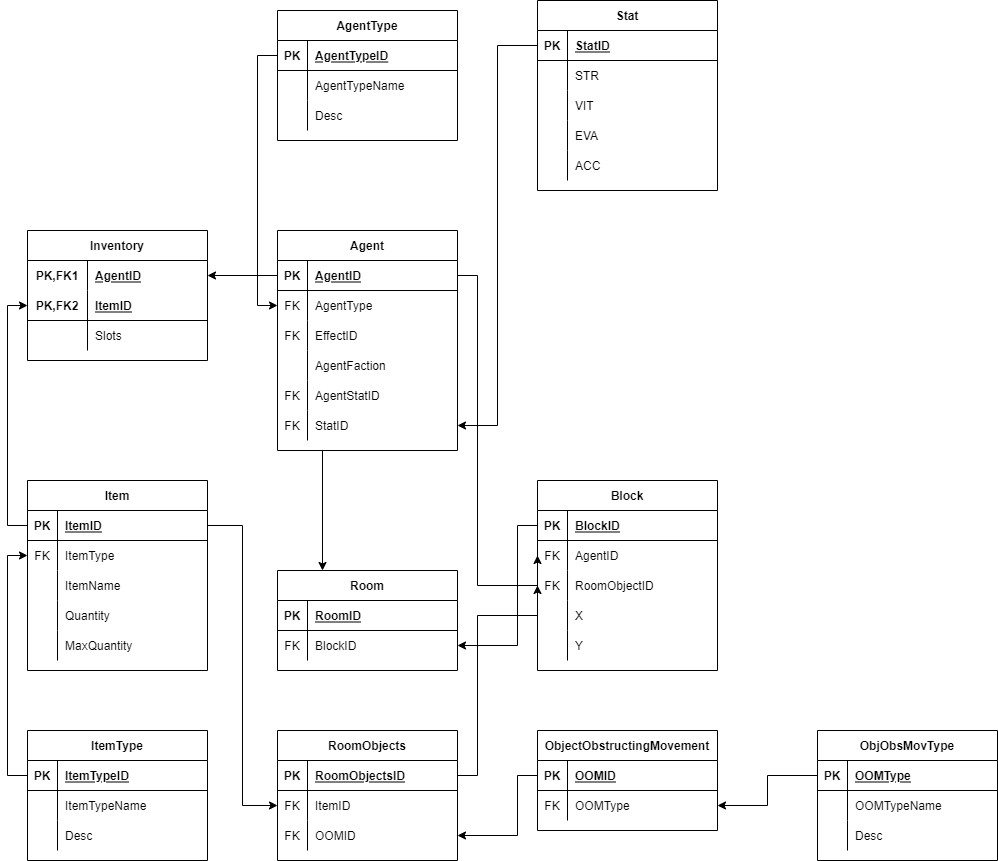
\includegraphics[width=\textwidth]{images/relaciosadatmodel7.png}
    \caption{Legelső tervezéshez tartozó relációsadatmodel}
    \label{fig:relmod}
\end{figure}

Ez még csak egy előzetes terv, melyhez képest a további, implementációhoz egyre közelebbi lépésekben bizonyos elemek változtak.

Először az ágensekhez tartozó statisztikák és az \textit{Inventory} került bele az ágensek adataiba. Az inventory-hoz relációs séma szerint egy külön táblára volt szükség. Ez több szempontból is indokoltnak látszott. Egyrészt az \textit{Inventory}-ban lévő elemek száma nem ismert előre (így nem volt lehetőség azokat közvetlenül, mezőként megadni), másrészt szükségesnek látszott a későbbiekre nézve felkészülni arra, hogy közvetlenül az elemekre is lehessen szűrést végezni, például hogy van-e olyan ágens, amelyik rendelkezik egy adott tárggyal.

A szobák adatainak kezelése nem ilyen formában valósult meg. A sémában szereplő változat még azt az állapotot tükrözi, amelyben minden szobához közvetlenül, egyesével történik a blokkok hozzárendelése. A modell kialakításánál a mátrixos reprezentáció jóval egyszerűbb, kézenfekvőbb megoldásnak tűnt.

A szobákban lévő objektumok végül úgy lettek megoldva, hogy a térképen vannak elhelyezve koordináta alapján, és a hozzátartozó típusok is magukba az objektumokba kerültek. Koncepcionálisan a séma ugyan megvalósítható lett volna ebben a formában is, de a térképre jellemző kialakítás előnyösebbnek bizonyult.

A relációs sémában kézenfekvőnek tűnt minden rekordhoz egyedi azonosítót rendelni. Az objektum orientált modell ehhez képest egyszerűsödött, abban már a tárolók (többségében listák) indexei elegendőek voltak.

A szimulációs környezet tervezésénél nem volt cél az, hogy egy konkrét állapotot szerializálni és deszerializálni lehessen, továbbá az sem, hogy az állapot több számítógép között megoldható legyen. Mindkét eset egy reális további fejlesztési lehetőségként felmerülhet, amelyhez a relációs modell használata az adatok leírásához és tárolásához már szükséges lehet.

\Section{Osztályok és kapcsolataik}

A keretrendszer a széles körben elterjedt objektum orientált tervezési módszereknek megfelelően készült. Az alkalmazáshoz tartozó osztályok és azok kapcsolatai \aref{fig:UML}. ábrán láthatók.

\newpage

\begin{figure}[!ht]
    \centering
    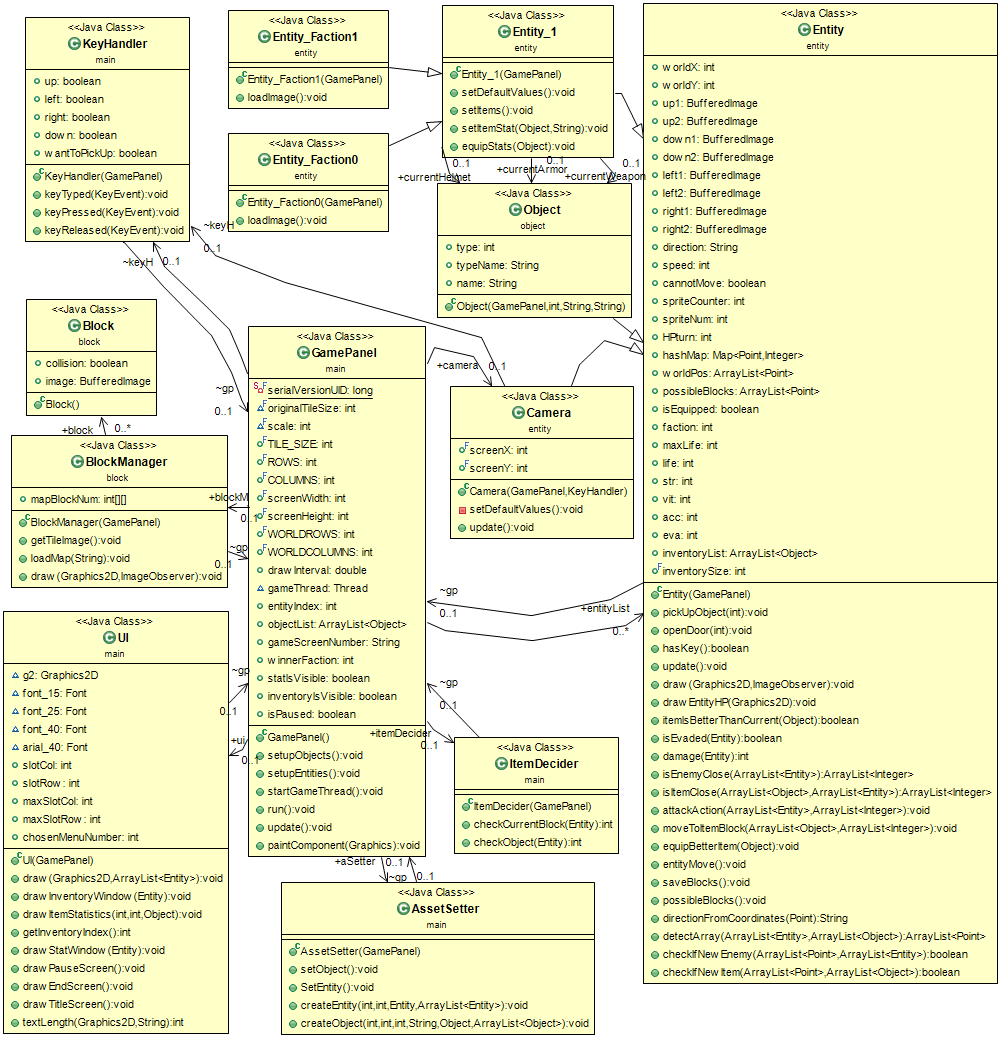
\includegraphics[width=\textwidth]{images/UML.png}
    \caption{A keretrendszerhez tartozó osztályok}
    \label{fig:UML}
\end{figure}

\noindent A következő szakaszok részletesen kitérnek ezek szerepére.

\subsection{KeyHandler}

A \textit{KeyHandler} osztály felel a kamera mozgatásáért, a játékmenet elinditásáért/megállításért, UI elemek használatáért, 
mint például az \textit{Inventory} és \textit{Statistics} oldal megnyitása/bezárása.

Az adatai között külön logikai változóként szerepelnek az irányításért felelős kurzor billentyűk aktuális állapotai. Ez ahhoz szükséges, hogy a program egészére nézve aszinkron módon elérhető legyen azok állapota, mivel egyébként csak események formájában lennének jelen a rendszerben.

\subsection{Block}

A \textit{Block} osztály a szimulátorban szereplő négyzet alakú blokkokat reprezentálja. Aránylag kevés adattal rendelkezik, mivel azok a rendszer többi eleméhez kerültek átcsoportosításra (például az entitásokhoz).

Az osztályhoz tartozik egy \textit{BufferedImage} típusú adattag. Ez magának a blokknak a megjelenítéséhez szükséges kirajzolható raszteres képet tárolja.

\subsection{BlockManager}

\textit{Block} típusok definiálása, tulajdonságok megadása és képek beolvasása a res mappából.

Egy \texttt{txt} kiterjesztésű fájlból beolvas egy $50 \times 50$-es mátrixot, amelyben minden elem 0, 1 vagy 2 egész értéket vehet fel. Az elemek szóközzel vannak elválasztva.

A \textit{BlockManager} osztály felelős azért, hogy megrajzolja a térképet megvalósító blokkok kinézetet az alapján, hogy hol helyezkedik el a térképen és hogy milyen blokk kép tartozik a blokk típusához. Ehhez szüksége van arra, hogy be tudja tölteni a térképeket és a képeket a \textit{loadMap} és a \textit{getTileImage} metódusai segítségével.

\subsection{GamePanel}

Tartalmazza a képernyő felbontásának adatait, a blokkok méretét, az ágens listát és az objektumok listáját. (Utóbbiak neve nagy betűvel szerepel, mivel konstans értéknek tekinthetők az alkalmazás szempontjából, de lényegesnek tünt a kód érthetősége és a későbbi fejlesztések szempontjából nevesíteni őket.)

A \textit{GamePanel} osztály segítségével inicializálódik a kezdő képernyő az alkalmazás elindítása után.
Tartalmazza azokat a függvényeket, amelyek kezelik az ágens és objektum létrehozását. Ezek hívódnak meg a \textit{main} metódusban. Továbbá ez felelős a \textit{UI} elemek, az ágensek és tárgyak megrajzolásáért.

\subsection{Camera}

Kamera kezdő helyzetét, egy lépés távolságát (blokkokban) határozza meg.
Kezeli továbbá a képernyő koordinátáit is.

\subsection{AssetSetter}

Az objektumok és ágensek elhelyezésért felelős.
Két fontosabb függvényt tartalmaz.
\begin{itemize}
    \item A \textit{setEntity} metódus szolgál minden ágens létrehozásának a tárolására.
    \item A \textit{setObject} metódus szolgál minden objektum létrehozásának a tárolására.
\end{itemize}

amelyek felelősek az ágensek és a térképen minden megtalálható objektum létrehozásáért a szimuláció elején.

\subsection{UI}

A \textit{gameScreenNumber} változó által tárolt 3 fő képernyő megjelenítését tartalmazza: kezdő képernyő (\textit{title}),
játékmenet (\textit{normal}) és végsőképernyő (\textit{endscreen}).
Itt történnek a képernyőre való szöveg kiírások is.
\textit{Inventory} és \textit{Statistics} ablak megjelenítését is tartalmazza.

\subsection{Entity}

A következő fontosabb ágens adatokat tárolja:
\begin{itemize}
    \item $X$ és $Y$ koordináta: a térképen lévő helyzetét jelentő értékek
    \item \textit{HPturn}: Azt az érték tárolja, hogy hány kör múlva lesz életerő regenerálódás.
    \item Alapstatisztikák: Életerő, erő, kitartás, kitérés, pontosság.
    \item \textit{InventorySize}: Az \textit{Inventory}-ban maximálisan elhelyezhető objektumok száma.
    \item Irány: Meghatározza, hogy melyik irányba néző képet kell betöltenie.
    \item Gyorsaság: Lépésenként mennyi utat tesz meg, ez egy rögzített érték, amely egy blokknyi távolság.
\end{itemize}

\noindent Itt történik az ágensek :
\begin{itemize}
    \item életcsíkjának a megrajzolása,
    \item megrajzolása a képernyőre,
    \item által legutoljára felvett hordható tárgy statisztika vizsgálata,
    \item tárgy felvétele,
    \item támadása, kulcs használata és mozgása,
    \item találatának eldöntése és sebzés méretének a kiértékelődése,
    \item és objektumok észlelése,
    \item \textit{hashMap} értékeinek frissítése.
\end{itemize} 

\subsection{ItemDecider}

Két fontosabb függvényt tartalmaz, amely egy-egy indexet ad vissza az Entity osztálynak, amelyek által kiértékelődik az, hogy az ágensek akarnak-e felvenni tárgyat a saját blokkjukról vagy kinyitni egy ajtót egy nekik szomszédos blokkról.
Az egyik függvény azt vizsgálja, hogy van-e valamilyen objektum az ágens koordinátáján, a másik függvény azt vizsgálja, hogy van-e az ágens koordinátája
alatti, feletti, jobb oldali vagy baloldali szomszédján valamilyen objektum.

\subsection{Object}

Az \textit{objectek} osztálya, \textit{object} típusokat tartalmaz.
Az objektumok típusát, típus nevét és nevét tárolja. Ezek a változók fontosak a tárgyak vizsgálatánál ágens szempontból.
Ezek származtatásával jönnek létre az objektumok a térképen.

\subsection{Entity1}

Ágensek egyetlen típusának alap értékeinek definiálására szolgál.
Tartalmazza az ágensek kezdő felszereléseit, ezek a felszereléseknek a változói itt kapnak értéket.
És itt kerülnek felszerelésre az ágensre statisztikailag és kerülnek be az \textit{Inventory}-ba.

\subsection{EntityFaction0 és EntityFaction1}

A 0-ás és 1-es \textit{faction}-höz tartozó ágensek képeit tárolja, amelyeket láthatunk a szimulációban.
